\documentclass[spanish,notitlepage,letterpaper, 12pt]{article} % para articulo en castellano
\usepackage[ansinew]{inputenc} % Acepta caracteres en castellano
\usepackage[spanish]{babel} % silabea palabras castellanas
\usepackage{url}
\usepackage{amsmath}
\usepackage{amsfonts}
\usepackage{float}
\usepackage{amssymb}
\usepackage[colorlinks=true,urlcolor=blue,linkcolor=blue]{hyperref} % navega por el doc
\usepackage{graphicx}
\usepackage{geometry}      % See geometry.pdf to learn the layout options.
\geometry{letterpaper}                   % ... or a4paper or a5paper or ...
%\geometry{landscape}                % Activate for for rotated page geometry
%\usepackage[parfill]{parskip}    % Activate to begin paragraphs with an empty line rather than an indent
\usepackage{epstopdf}
\usepackage{fancyhdr} % encabezados y pies de pg
\usepackage{pgf,pgfarrows,pgfnodes}
\usepackage{graphicx}

\renewcommand{\spanishtablename}{Cuadro}

\pagestyle{fancy}
\chead{\bfseries Tarea 2}
\lhead{} % si se omite coloca el nombre de la seccion
\rhead{ }
\lfoot{\it }
\cfoot{}
\rfoot{\thepage}

\voffset = -0.25in
\textheight = 9.0in
\textwidth = 6.5in
\oddsidemargin = 0.in
\headheight = 20pt
\headwidth = 6.5in
\renewcommand{\headrulewidth}{0.5pt}
\renewcommand{\footrulewidth}{0,5pt}
\DeclareGraphicsRule{.tif}{png}{.png}{`convert #1 `dirname #1`/`basename #1 .tif`.png}

\begin{document}
\title{Tarea 2 \\ An�lisis de texto}

\author{
\textbf{Erick Cervantes Mendieta} \\
\vspace{0.5cm}
\textnormal{Matr�cula: 2032430}\\
\textit{Modelos Probabilistas Aplicados}}
\date{Septiembre 2020}

\maketitle

%------------------------------------------------

\section{Presentaci�n de los datos}

Para esta tarea se analiz� el libro titulado ``The Singing Mouse Stories", el cual se encuentra disponible de manera gratuita en el sitio Web: \emph{Project Gutenberg} \cite{Mouse}. Se utilizaron algunas t�cnicas para an�lisis de texto, como lo es las frecuencias de las letras y de las palabras, ideal para identificar r�pidamente los temas comunes, y por otra parte, el agrupamiento de palabras, ya que a veces un grupo de palabras puede proporcionar una mejor perspectiva que una sola palabra.\\

En el cuadro \ref{t1} se pueden observar las cinco letras m�s utilizadas en el libro y en el cuadro \ref{t2}, se pueden observar las palabras m�s frecuentes en el texto.

\begin{table}[]
\centering
\caption{Letras m�s utilizadas en el libro}
\vspace{0.3 cm}
\begin{tabular}{c|c}
 Letra & Frecuencia \\
 \hline
  e & 10395 \\
  t & 7894 \\
  a & 6741 \\
  o & 6306 \\
  n & 5857 \\
\end{tabular}
\label{t1}
\end{table}

\begin{table}[]
\centering
\caption{Palabras m�s utilizadas en el libro}
\vspace{0.3 cm}
\begin{tabular}{c|c}
 Letra & Frecuencia \\
 \hline
  the & 1775 \\
  and & 895 \\
  of & 731 \\
  in & 367 \\
  it & 350 \\
\end{tabular}
\label{t2}
\end{table}

\section{An�lisis de los datos}

Tanto las palabras como las letras utilizadas en la redacci�n del libro fueron analizadas, en el sentido de que se pudieron ordenaran seg�n la frecuencia con la que aparecieron, por otra parte, los d�gitos como las preposiciones, los art�culos y las conjunciones fueron excluidos(as) del an�lisis, ya que estos no aportaban gran informaci�n.\\

La figura \ref{f1} muestra el n�mero de veces que fueron utilizadas las letras del abecedario en el texto en orden descendente, en donde se puede  observar que la letra m�s utilizada fue la \textbf{e} y la menos utilizada fue la \textbf{x}. \\

\begin{figure}[]
\begin{center}
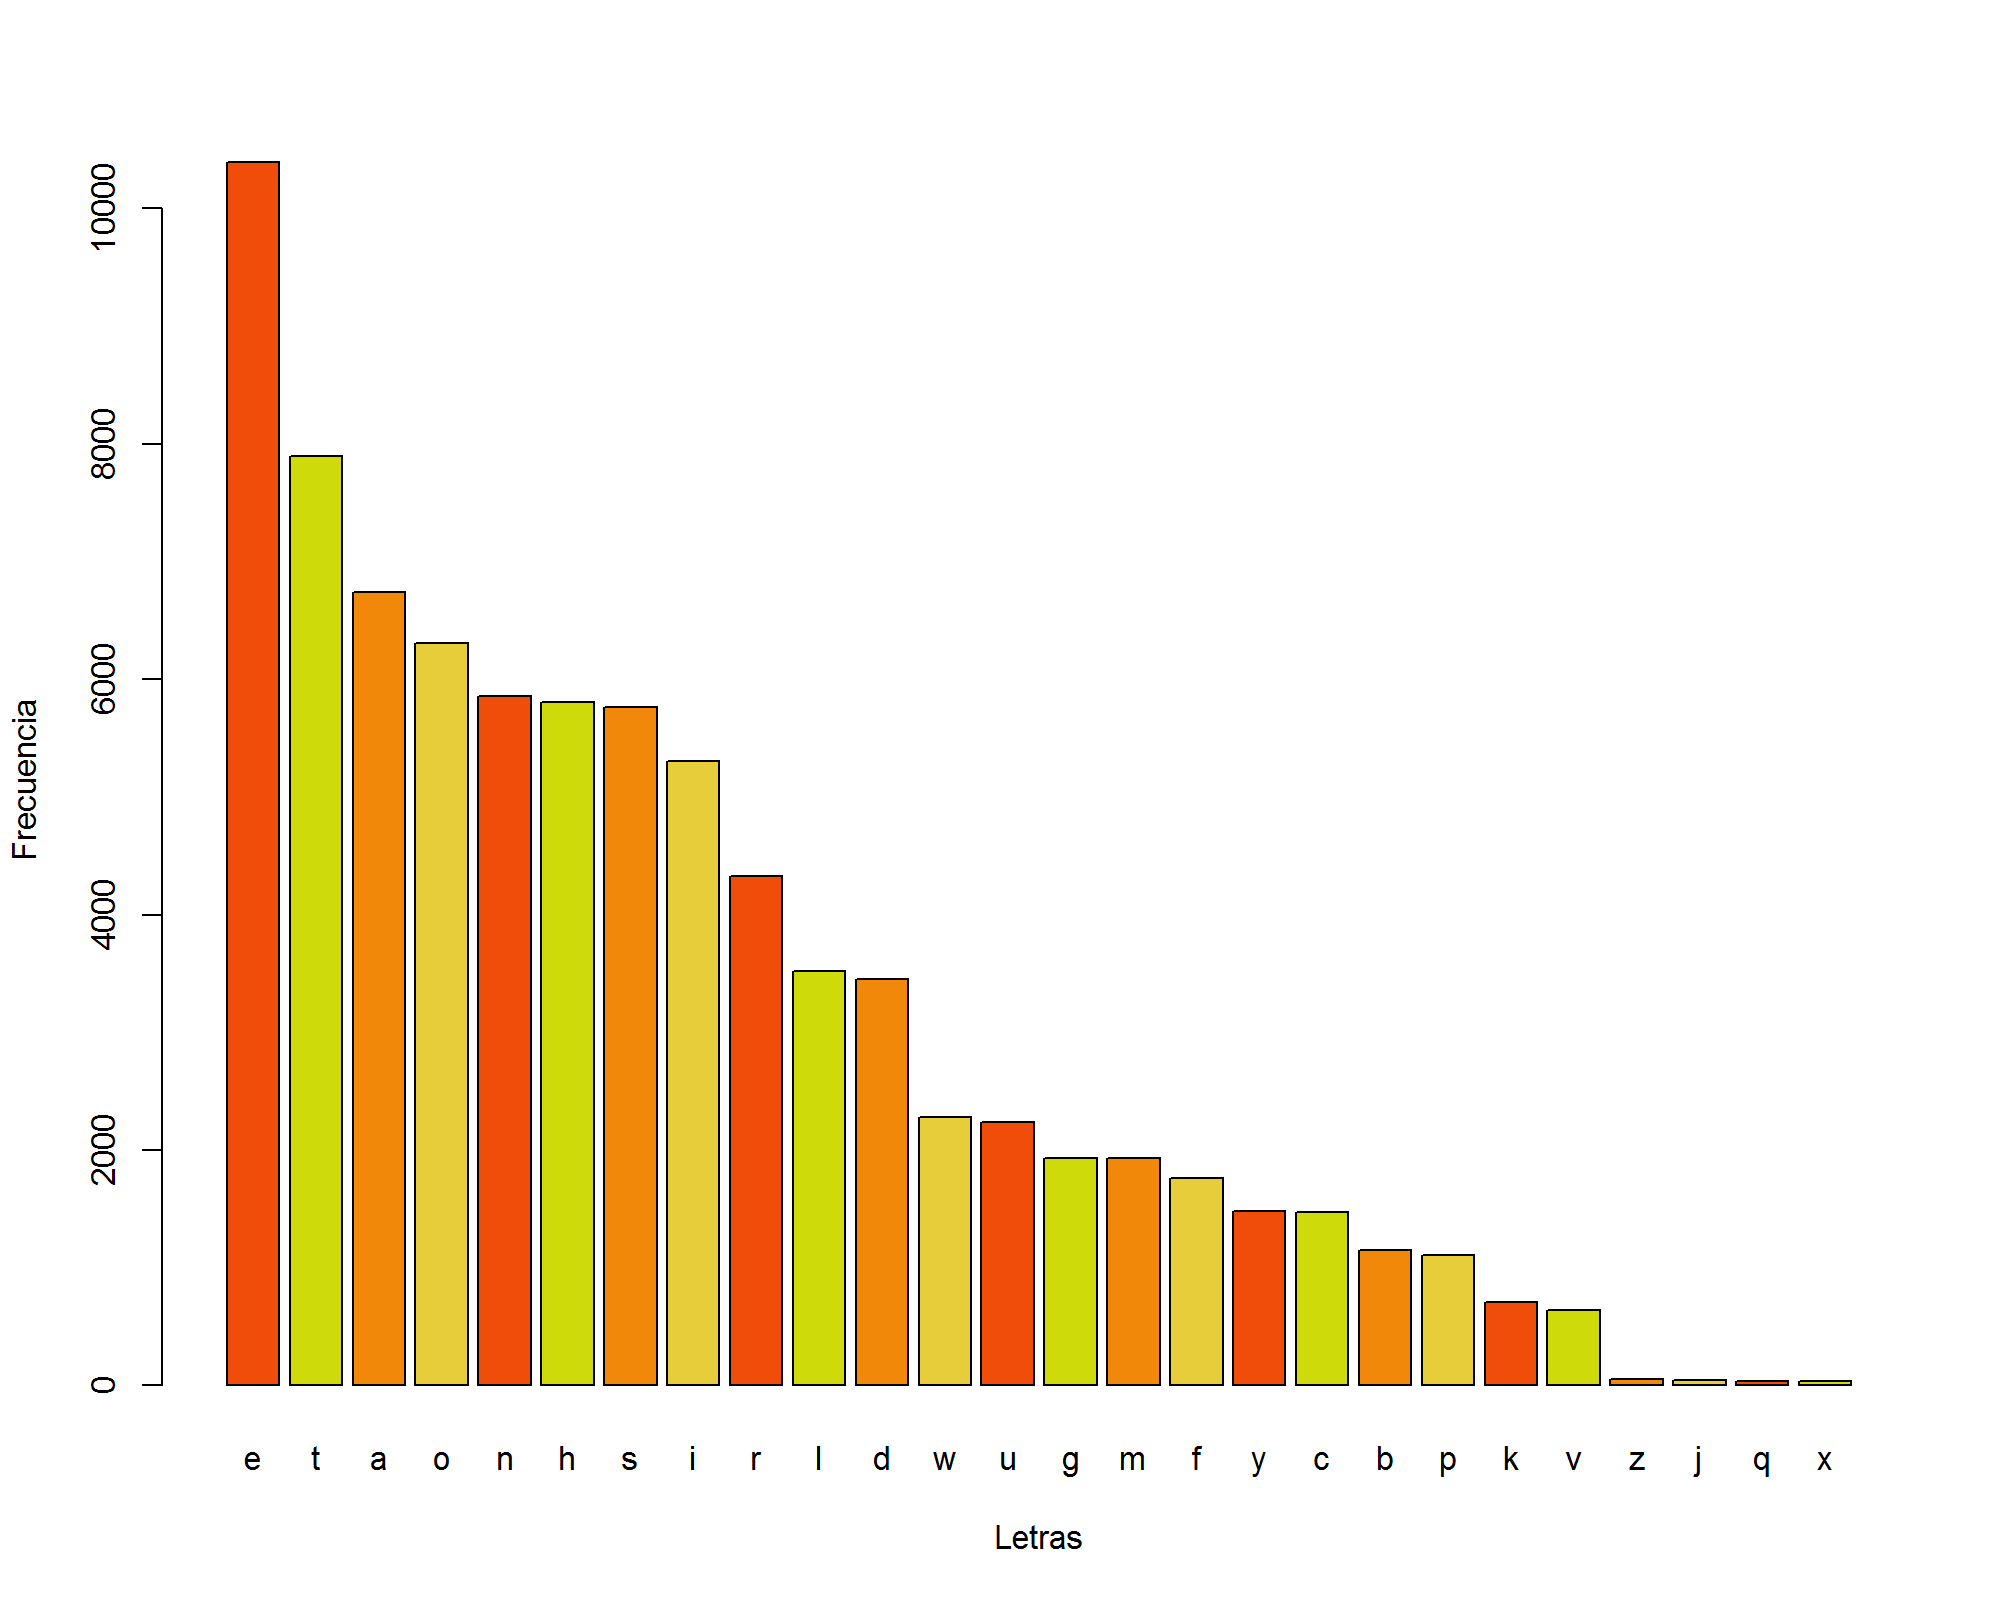
\includegraphics[width=16 cm]{FigModeloReporte/T2_letras.png}
\caption{Frecuencia de las letras utilizadas en el texto}\label{f1}
\end{center}
\end{figure}

En la figura \ref{f2} se pueden visualizar las palabras cuya frecuencia es mayor a cien, es decir, estas palabras aparecieron m�s de cien veces en el texto del libro, el listado es peque�o debido al tama�o del texto. Se observa que la palabra m�s utilizada fue el art�culo \textbf{the}, seguida de la conjunci�n \textbf{and}, y en tercer lugar la preposici�n \textbf{of}, estas palabras son conocidas como \emph{palabras huecas} \cite{mendoza2018}, ya que aportan poca informaci�n sem�ntica. Afortunadamente el programa R (Versi�n 4.0.2) \cite{LenguajeR} nos ofrece una herramienta para eliminar este tipo de palabras, lo que me permiti� poder obtener bigramas para poder extraer informaci�n relevante del texto.\\

\begin{figure}[]
\begin{center}
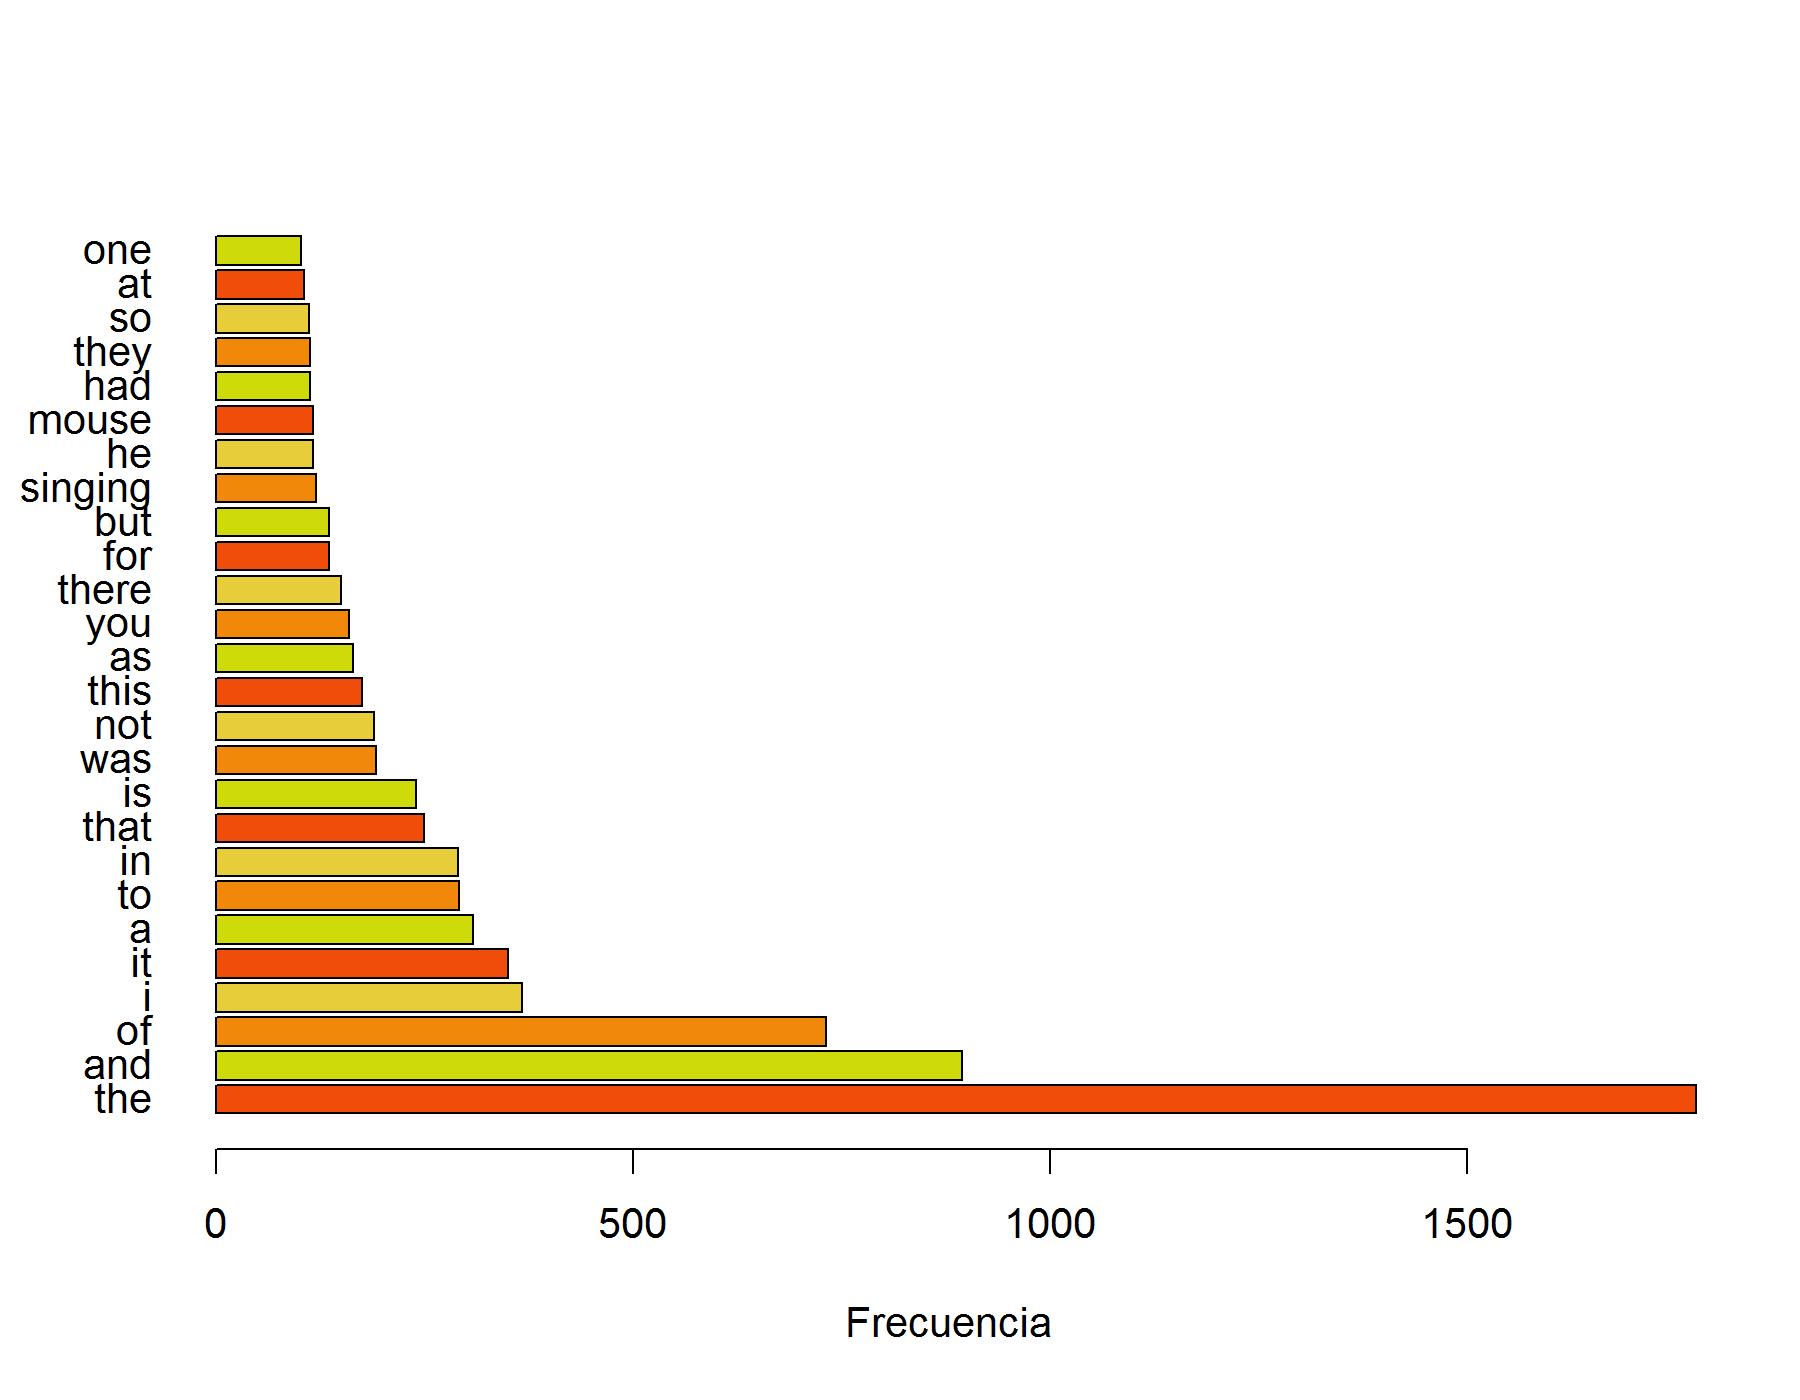
\includegraphics[width=16 cm]{FigModeloReporte/T2_palabras.png}
\caption{Frecuencia de las palabras m�s utilizadas en el texto}\label{f2}
\end{center}
\end{figure}

La figura \ref{f3} expone una red sem�ntica con los bigrama obtenidos, los cuales no contienen palabras huecas. Esta red muestra la intensidad con la que se relacionan las palabras, es decir, la frecuencia con la que parejas de palabras aparecen en el texto. De dicha figura, podemos observar que aparece la palabra \emph{singing mouse}, lo que no da la referencia al personaje principal (debido al t�tulo tambi�n), otro conjunto de palabras que me llam� la atenci�n fue \emph{lake belle marie}, por lo que supongo la historia se desarrolla cerca de un lago. As� mismo, \emph{little river} y \emph{delectable mountains} nos hacen sospechar, que la historia se desarrolla cerca de un paisaje lleno de naturaleza.

\begin{figure}[]
\begin{center}
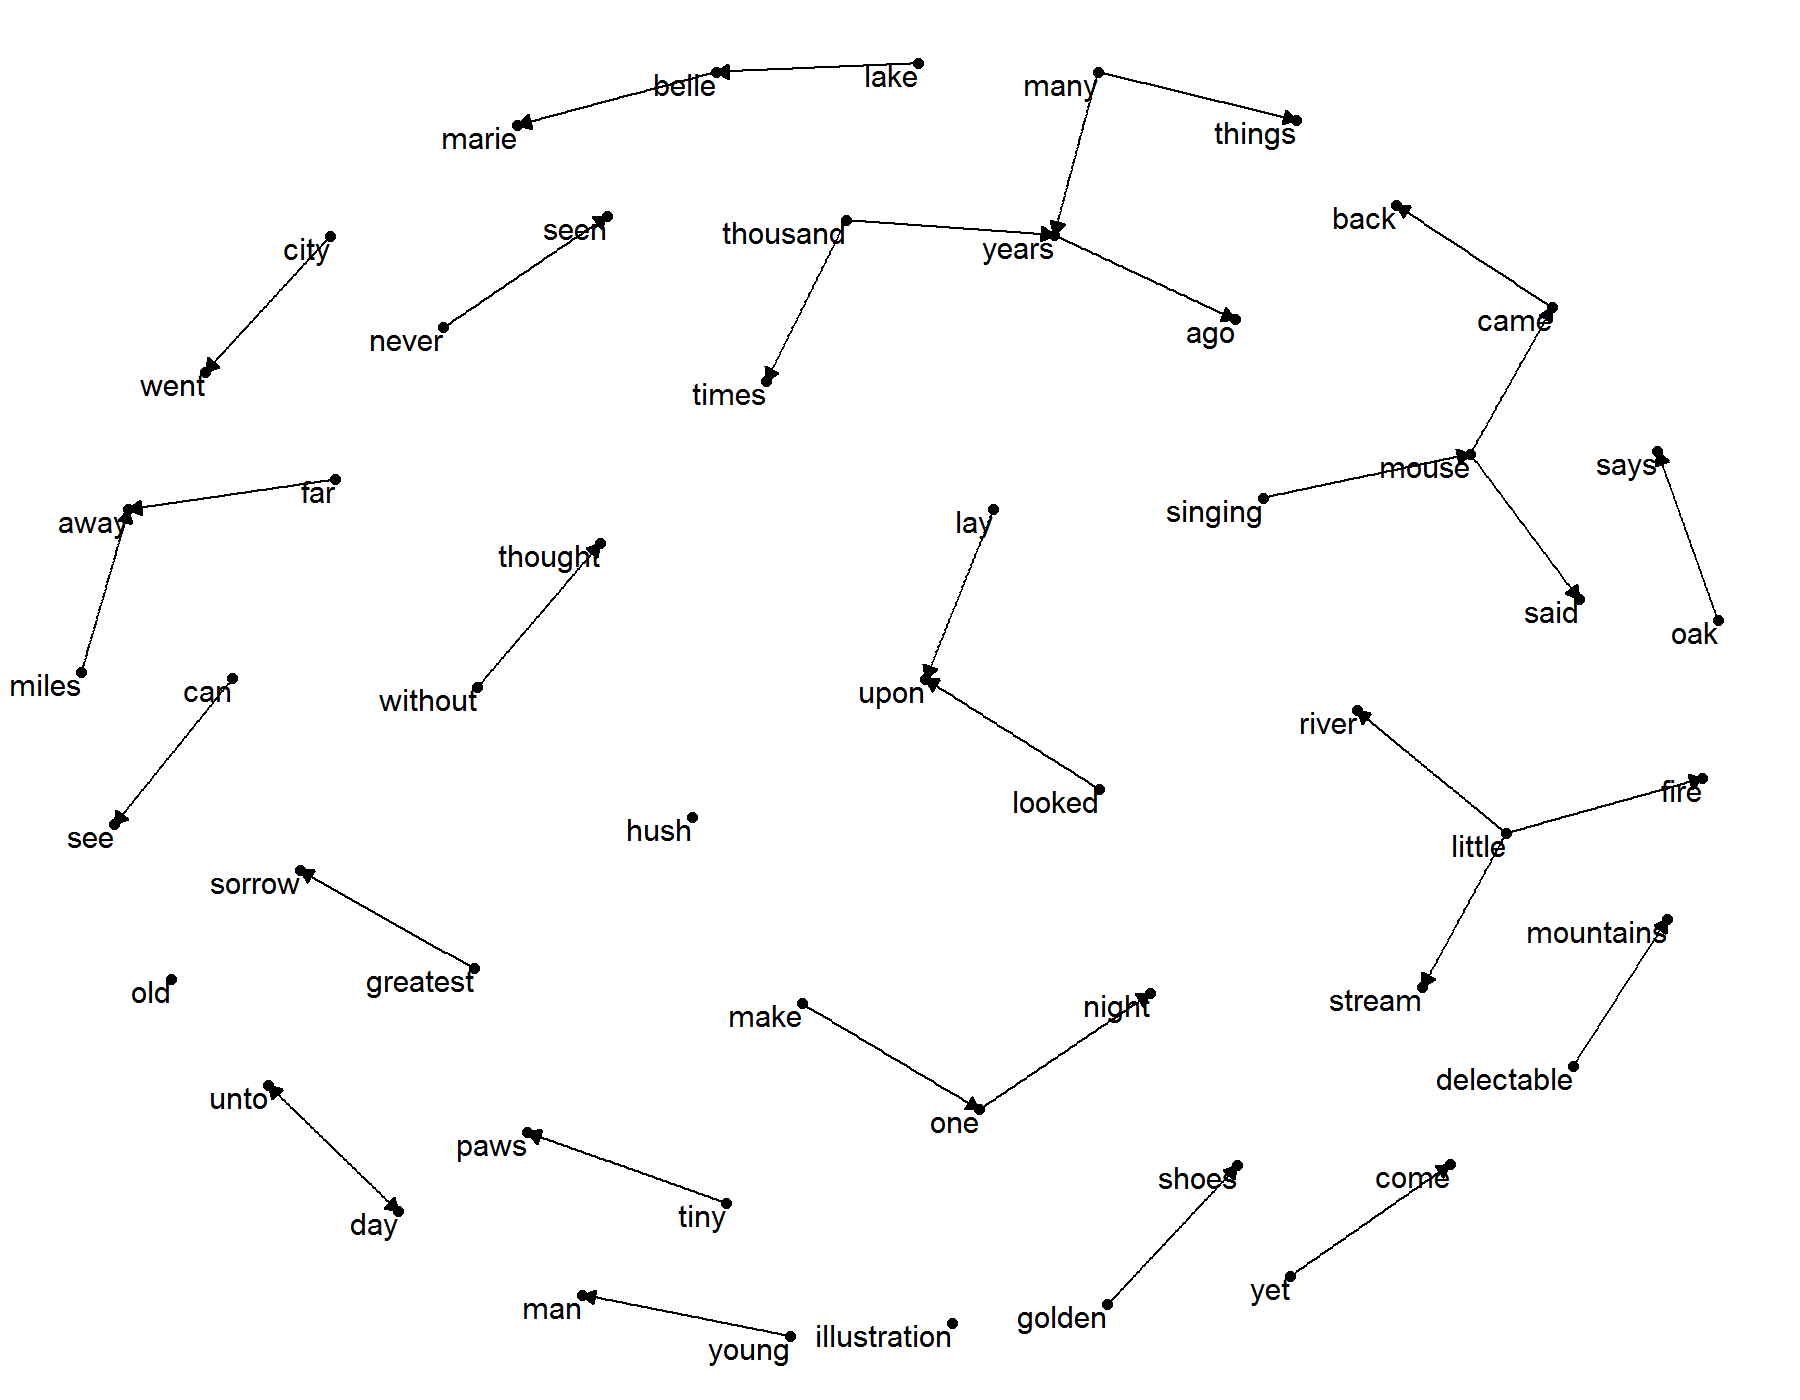
\includegraphics[width=16 cm]{FigModeloReporte/T2_bigrama.png}
\caption{Red sem�ntica de parejas de palabras utilizadas en el texto}\label{f3}
\end{center}
\end{figure}

\bibliographystyle{plain}
\bibliography{MiBiblio}

\end{document} 